\documentclass[tikz]{standalone}
\usepackage{pgfplots}
%\pgfplotsset{compat=1.18}

\begin{document}
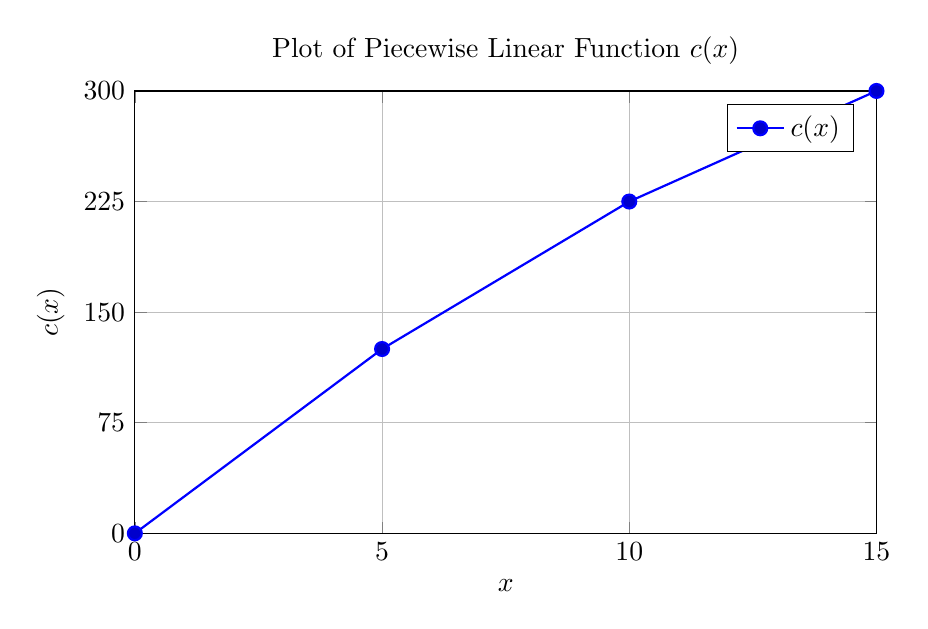
\begin{tikzpicture}
\begin{axis}[
  width=11cm, height=7.2cm,
  title={Plot of Piecewise Linear Function $c(x)$},
  xlabel={$x$}, ylabel={$c(x)$},
  xmin=0, xmax=15, ymin=0, ymax=300,
  xtick={0,5,10,15},
  ytick={0,75,150,225,300},
  grid=both,
  legend pos=north east,
  legend cell align=left
]
  % polyline with circular markers
  \addplot+[thick, mark=*, mark size=2.5pt]
    coordinates {(0,0) (5,125) (10,225) (15,300)};
  \addlegendentry{$c(x)$}
\end{axis}
\end{tikzpicture}
\end{document}
